
% We evaluate MoIE on five datasets - 1) bird classification using CUB-200 \cite{wah2011caltech} dataset, 2) animal classification using Animals with Attributes2 (Awa2) dataset \cite{xian2018zero}, 3) skin lesion classification using the HAM10000 dataset \cite{tschandl2018ham10000}, 4) . 5) classification of the disease Effusion using the MIMIC-CXR dataset \cite{12_johnsonmimic}. 
We perform experiments on a variety of vision and medical imaging datasets to show that 1) MoIE captures a diverse set of concepts, 2) the performance of the residuals degrades over successive iterations as they cover ``harder'' instances, 3) MoIE does not compromise the performance of the Blackbox, 4) MoIE achieves superior performances during test time interventions, and 5) MoIE can fix the shortcuts using the Waterbirds dataset \cite{sagawa2019dro}. We repeat our method until MoIE covers at least 90\% of samples or the final residual's accuracy falls below 70\%. Refer to~\cref{tab:dataset} for the datasets and Blackboxes experimented with. For ResNets and Inception, we flatten the feature maps from the last convolutional block to extract the concepts. For VITs, we use the image embeddings from the transformer encoder to perform the same. We use SIIM-ISIC as a real-world transfer learning setting, with the Blackbox trained on HAM10000 and evaluated on a subset of the SIIM-ISIC Melanoma Classification dataset~\cite{yuksekgonul2022post}.~\cref{app:dataset} and~\cref{app:g} expand on the datasets and hyperparameters.
% \textbf{Training configurations:} CUB-200 and Awa2 use ResNet101~\cite{he2016deep} and Vision Transformer (VIT)~\cite{wang2021feature} as blackboxes. HAM10000 and MIMIC-CXR use Inception~\cite{szegedy2015going} and Densenet121~\cite{huang2017densely}, respectively. For CUB-200, we use 6 experts each for both VIT and ResNet-based Blackboxes. For Awa2, we utilize 4 and 6 experts for ResNet-101 and VIT, respectively. For skin lesion classification (both HAM10000 and SIIM-ISIC) and MIMIC-CXR, we use 6 and 3 experts, respectively. Appendices~\ref{app:dataset} and~\ref{app:g} detail the datasets and hyperparameters.

\begin{figure*}[ht]
\vskip 0.2in
\begin{center}
\centerline{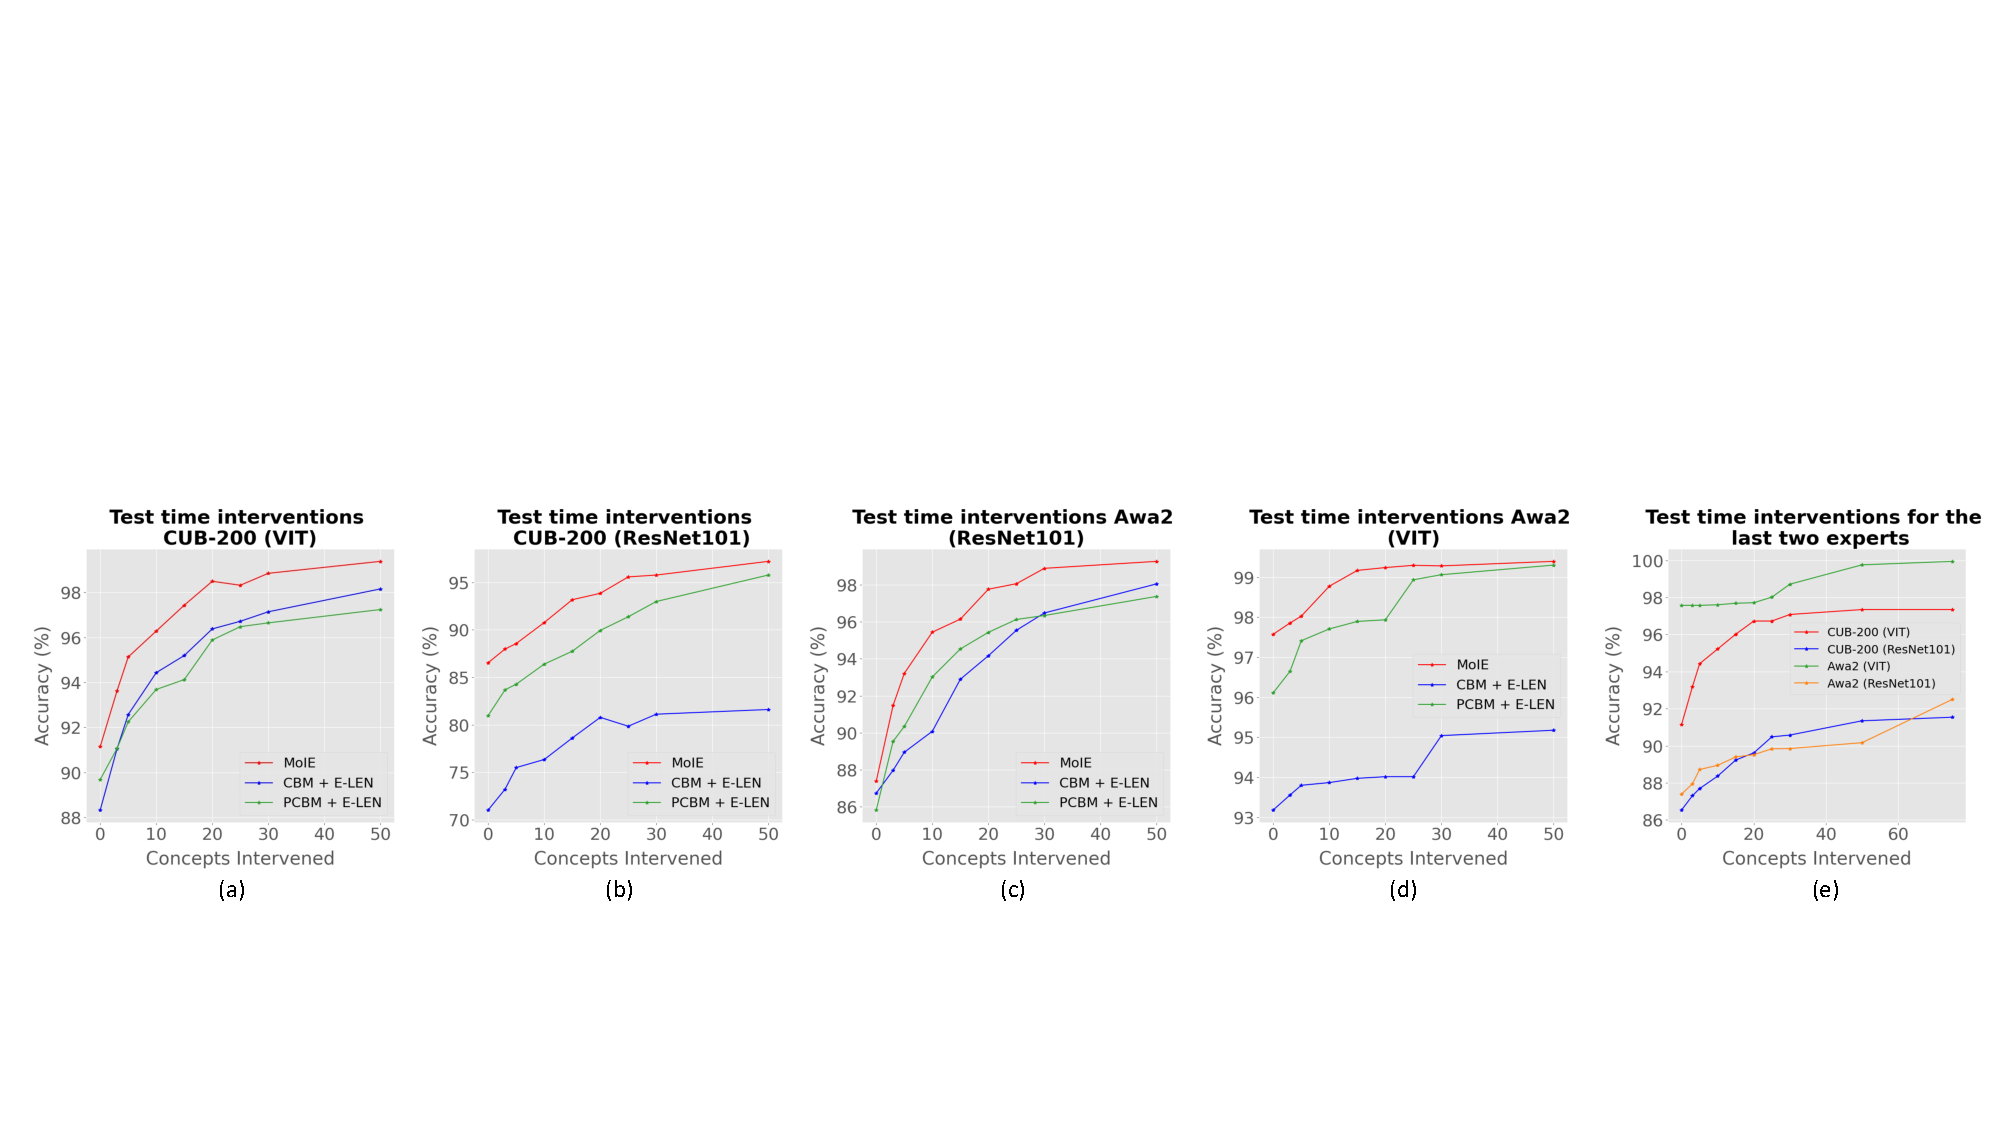
\includegraphics[width=\linewidth]{figures/main/TTI_all.pdf}}
\caption{Across architectures test time interventions of concepts  on all the samples \textbf{(a-d)}, on the ``hard'' samples \textbf{(e)}, covered by only the last two experts of MoIE. 
% All the plots mark the first point on the x-axis as "0," indicating the original model's performance with no intervention
}
\label{fig:tti}
\end{center}
\vskip -0.2in
\end{figure*}

% \begin{figure}[h]
% % \vskip 0.1in
% \begin{center}
% \centerline{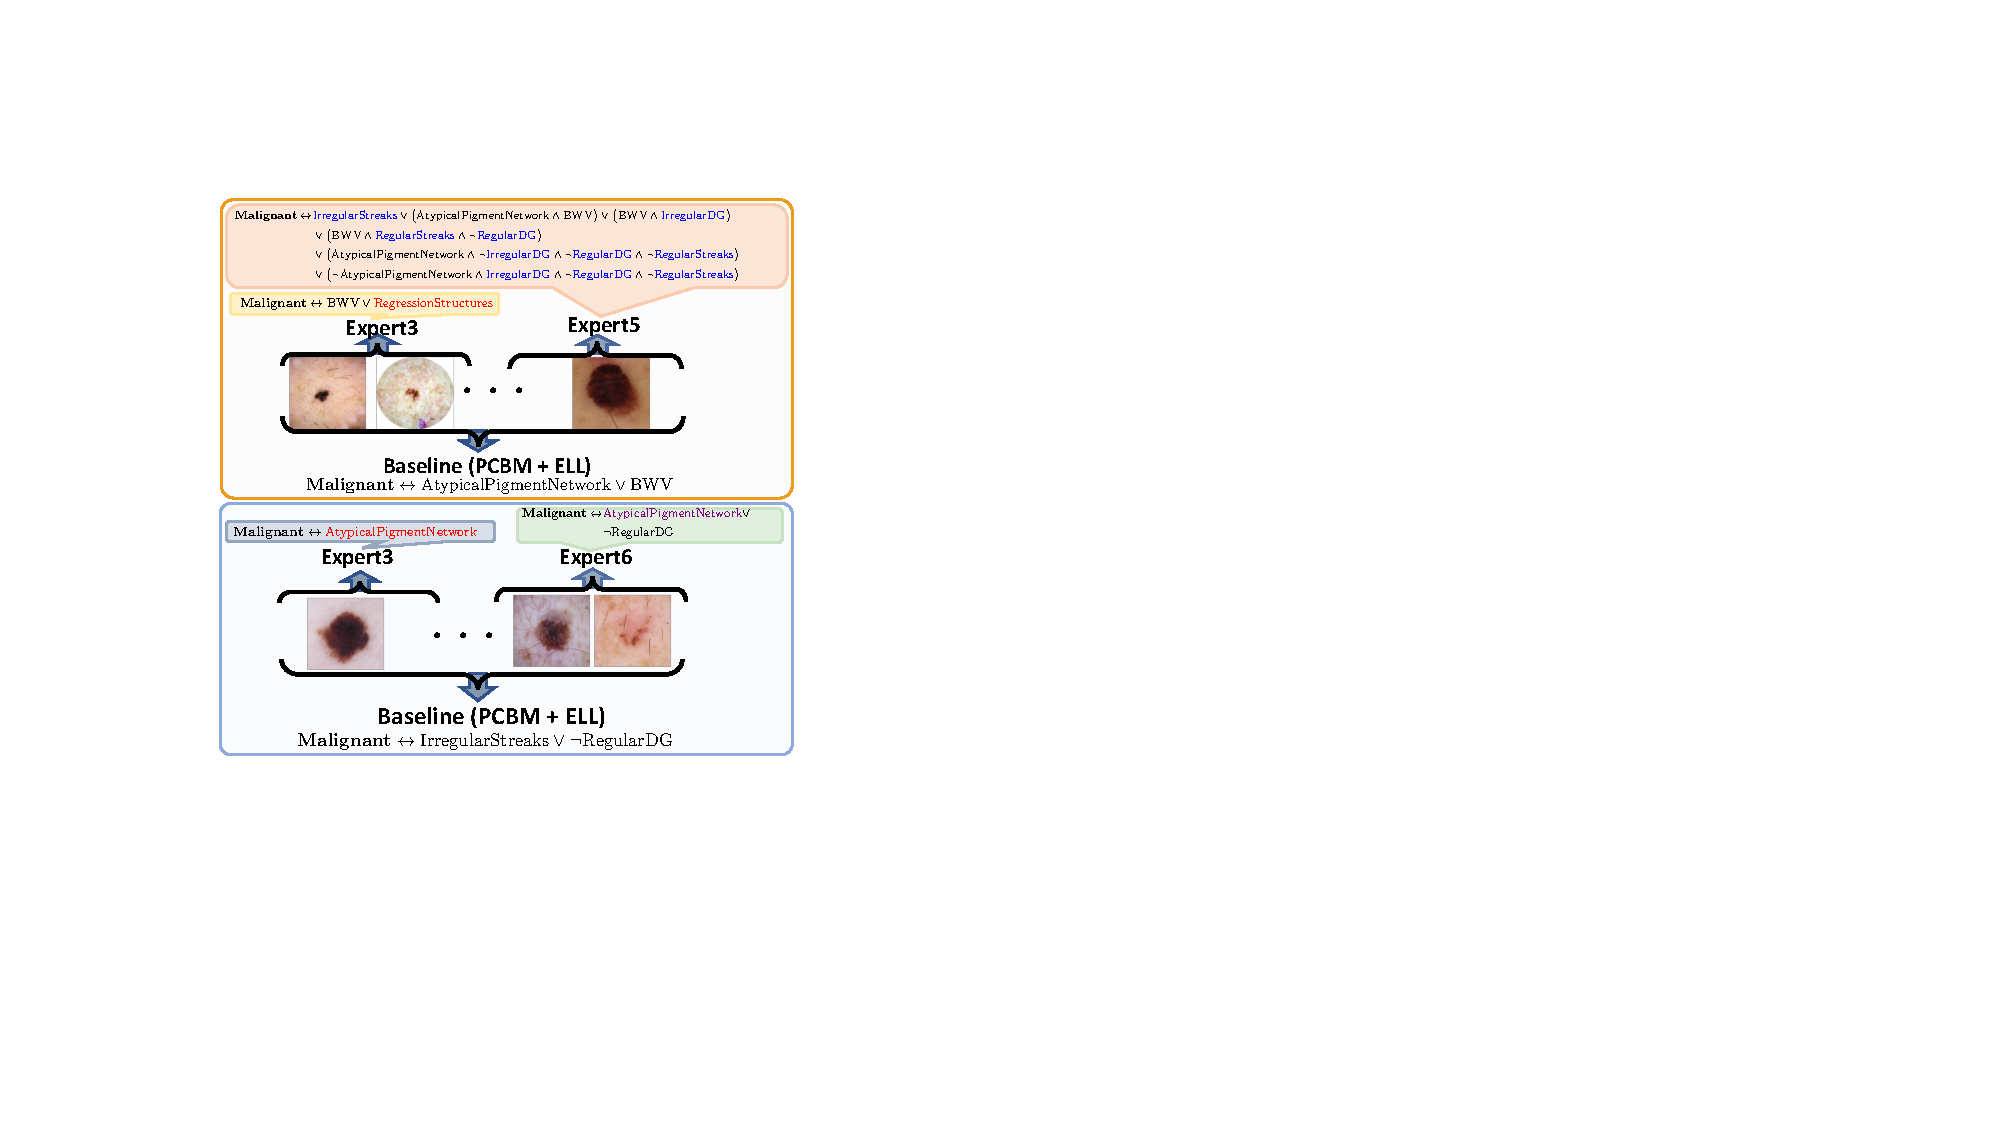
\includegraphics[width=\columnwidth]{figures/main/Local.pdf}}
% \caption{Flexibility of FOL explanations by MoIE compared to the PCBM + E-LEN baselines for HAM10000 (\emph{top}) and ISIC (\emph{down})  to classify Malignant lesion. We highlight unique concepts for experts 3, 5 and 6 in \emph{red}, \emph{blue} and \emph{violet} respectively.}
% \label{fig:local_awa2_skin}
% \end{center}
% \vskip -0.23in
% \end{figure}

\begin{figure}[h]
% \vskip 0.1in
\begin{center}
\centerline{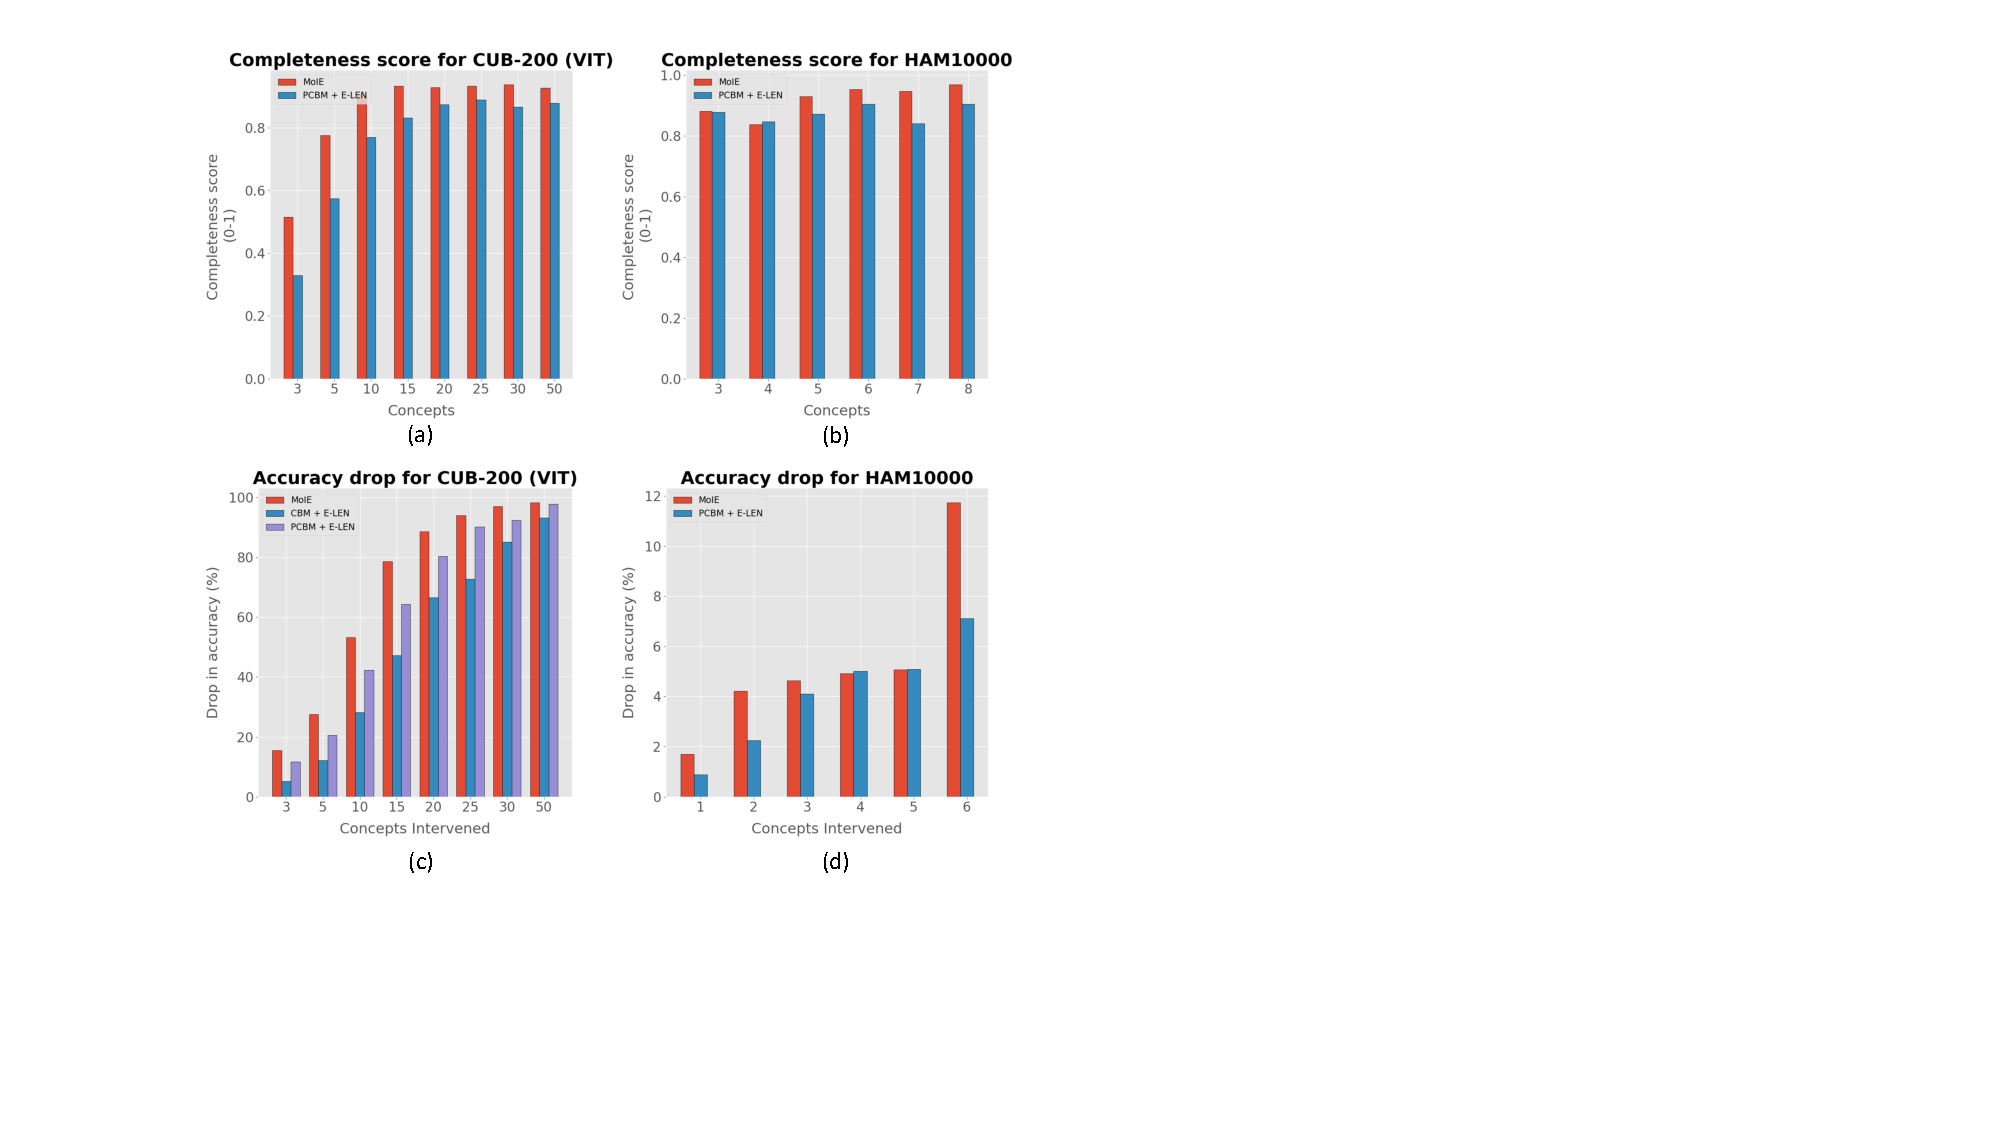
\includegraphics[width=\columnwidth]{figures/main/CUB_HAM.pdf}}
\caption{Quantitative validation of the extracted concepts and test time interventions. \textbf{(a-b)} 
Completeness scores of the models for a varying number of top concepts. (\textbf{c-d)} Drop in accuracy compared to the original model after zeroing out the top significant concepts iteratively. The highest drop for MoIE indicates that MoIE selects more instance-specific concepts than generic ones by the baselines. 
% All the plots mark the first point on the x-axis as "0," indicating the original model's performance with no intervention
}
\label{fig:valid_concepts}
\end{center}
\vskip -0.2in
\end{figure}


\textbf{Baselines:}
We compare our methods to two concept-based baselines -- 1) interpretable-by-design and 2) posthoc. They consist of two parts: a) a concept predictor $\Phi: \mathcal{X} \rightarrow \mathcal{C}$, predicting concepts from images; and b) a label predictor $g: \mathcal{C} \rightarrow \mathcal{Y}$, predicting labels from the concepts. The end-to-end CEMs and sequential CBMs serve as interpretable-by-design baselines. Similarly, PCBM and PCBM-h serve as post hoc baselines. Convolution-based $\Phi$ includes all layers till the last convolution block. VIT-based $\Phi$ consists of the transformer encoder block. The standard CBM and PCBM models do not show how the concepts are composed to make the label prediction. So, we create CBM + E-LEN, PCBM + E-LEN and PCBM-h + E-LEN by using the identical $g$ of MOIE (shown in~\cref{app:g}), as a replacement for the standard classifiers of CBM and 
PCBM. We train the $\Phi$ and $g$ in these new baselines to sequentially generate FOLs~\cite{barbiero2022entropy}. Due to the unavailability of concept annotations, we extract the concepts from the Derm7pt dataset~\cite{kawahara2018seven} using the pre-trained embeddings of the Blackbox~\cite{yuksekgonul2022post} for HAM10000. Thus, we do not have interpretable-by-design baselines for HAM10000 and ISIC.

